%----------------------------------------------------------------------------------------
%	PACKAGES AND THEMES
%----------------------------------------------------------------------------------------
\documentclass[aspectratio=169,xcolor=dvipsnames]{beamer}
\usetheme{SimplePlus}
\usepackage{ulem}
\usepackage{cancel} 
\usepackage{algorithm,algorithmic}
\usepackage{hyperref}
\usepackage{graphicx} % Allows including images
\usepackage{booktabs} % Allows the use of \toprule, \midrule and \bottomrule in tables

%----------------------------------------------------------------------------------------
%	TITLE PAGE
%----------------------------------------------------------------------------------------

\title[short title]{Acceleration and Stochastic Gradient Descent} % The short title appears at the bottom of every slide, the full title is only on the title page
\subtitle{}

\author[Hanchao] {Hanchao Zhang}

\institute[] % Your institution as it will appear on the bottom of every slide, may be shorthand to save space
{
% Your institution for the title page
}
\date{\today} % Date, can be changed to a custom date


%----------------------------------------------------------------------------------------
%	PRESENTATION SLIDES
%----------------------------------------------------------------------------------------

\begin{document}

\begin{frame}
    % Print the title page as the first slide
    \titlepage
\end{frame}

\begin{frame}{QUIZ}
\textbf{Momentum Gradient Descent}
\begin{align*}
	&w^{k+1} = w^k - \alpha z^{k+1}\\
	&z^{k+1} = \beta z^k + \nabla f(w^k)
\end{align*}

\begin{enumerate}
	\item Each step of momentum gradient descent should be closer to the optimal point compared to the gradient descent method with the same step size.  \\
	
	\begin{itemize}
		\item TRUE
		\item FALSE
	\end{itemize}

	\item In the setting of $f(w) = \frac{1}{2}w^T A w - b^Tw$, $A \succ 0$, only the largest eigenvalue of $A$ controls the convergence rate of momentum gradient descent.\\
	
	\begin{itemize}
		\item TRUE
		\item FALSE
	\end{itemize}

\end{enumerate}
	
	
\end{frame}

\begin{frame}{Overview}
    % Throughout your presentation, if you choose to use \section{} and \subsection{} commands, these will automatically be printed on this slide as an overview of your presentation
    \tableofcontents
\end{frame}

%------------------------------------------------
\section{Stochastic Gradient Descent}
%------------------------------------------------

\begin{frame}{Stochastic Gradient Descent}

\textbf{Motivation}

\begin{itemize}
	\item no access to full gradient
	\item to expensive to compute the full gradient
\end{itemize}

\textbf{Solution}

\begin{itemize}
	\item use the nosiy (stochastic) version of the gradient
	\begin{itemize}
		\item stochastic gradient descent
		\item random coordinate descent
	\end{itemize}
\end{itemize}
	
\end{frame}

%------------------------------------------------

\begin{frame}{Quick Peek -- Stochasitc Gradient Descent}

\textbf{Gradient Descent}

$$x^{k+1} = x^k - \eta \nabla f(x^k)$$

\textbf{Noisy Gradient}

$$\tilde g(x) = \nabla f(x) + \epsilon$$

where $\epsilon$ is zero mean, and 

$$E[\tilde g(x)] = \nabla f(x)$$
	
\end{frame}

%------------------------------------------------

\begin{frame}{Stochasitc Optimization}

\textbf{Original Optimization Problem}
\begin{align*}
	&\min f(x)\\
	&\text{subject to } \ x \in \mathcal X
\end{align*}
\textbf{Stochastic Optimization}
\begin{align*}
	&\min_x\  E_\xi [f(x; \xi )]\\
	&\text{subject to } \ x \in \mathcal X
\end{align*}
\textbf{Example -- Regression Problem}
\begin{align*}
	&\min_x \ E_\xi[(y - \xi^T x)^2]\\
	&\text{subject to } \ x \in \mathcal X
\end{align*}
\end{frame}

%------------------------------------------------

\begin{frame}{Example -- Regression Setting}

\begin{align*}
	&\min_x \ E_\xi[(y - \xi^T x)^2] \\
	=& \min_x \frac{1}{n} \sum_{i=1}^n (y_i - \xi_i^T x)^2\\
	=& \min_x f(x) = \frac{1}{n} \sum_{i=1}^n f_i(x)\\
	&\text{subject to } \ x \in \mathcal X
\end{align*}

\textbf{Gradient Descent}

\begin{equation*}
	x_{t+1} = x_t - \eta \nabla (\frac{1}{n} \sum_{i=1}^n f_i(x))
\end{equation*}
Very Expensive! Require Full pass over the data.	
\end{frame}

%------------------------------------------------

\begin{frame}{Example -- Stochastic Optmization}
\textbf{1. Stochastic Gradient}
\begin{align*}
	x \Longrightarrow \Box \Longrightarrow \xout{\nabla f(x)} \Longrightarrow \tilde g(x) = \nabla f_I(x)
\end{align*}

$$I \sim \text{uniform}(1, 2, \ldots, n)$$

\textbf{Q: is $\tilde g$ stochastic gradient? }


\begin{align*}
	E_I[\nabla f_I(x)] = \sum_{i = 1}^n \nabla f_i(x) \cdot \frac{1}{n} = \nabla f(x)
\end{align*}
	
\end{frame}

%------------------------------------------------

\begin{frame}{Example -- Stochastic Optmization}

\textbf{2. Random Coordinate Descent}

\begin{align*}
	x \Longrightarrow \Box \Longrightarrow \xout{\nabla f(x)} \Longrightarrow \tilde g(x) = d\nabla f_J(x) = d\cdot \begin{bmatrix}
		0 \\ \vdots \\ \frac{\partial f}{\partial x_j} \\ \vdots \\ 0
	\end{bmatrix}
\end{align*}

$$J\sim \text{uniform}(1, \ldots, d)$$
\textbf{Q: is $\tilde g$ stochastic gradient?}

\begin{align*}
	E_j[\tilde g(x)] = \sum_{j = 1}^n d \cdot  \nabla f_j(x) \cdot \frac{1}{d} = \nabla f(x)
\end{align*}

\end{frame}

%------------------------------------------------

\begin{frame}{SGD -- Role of Variance}
\textbf{Regression Setting}

\begin{center}
	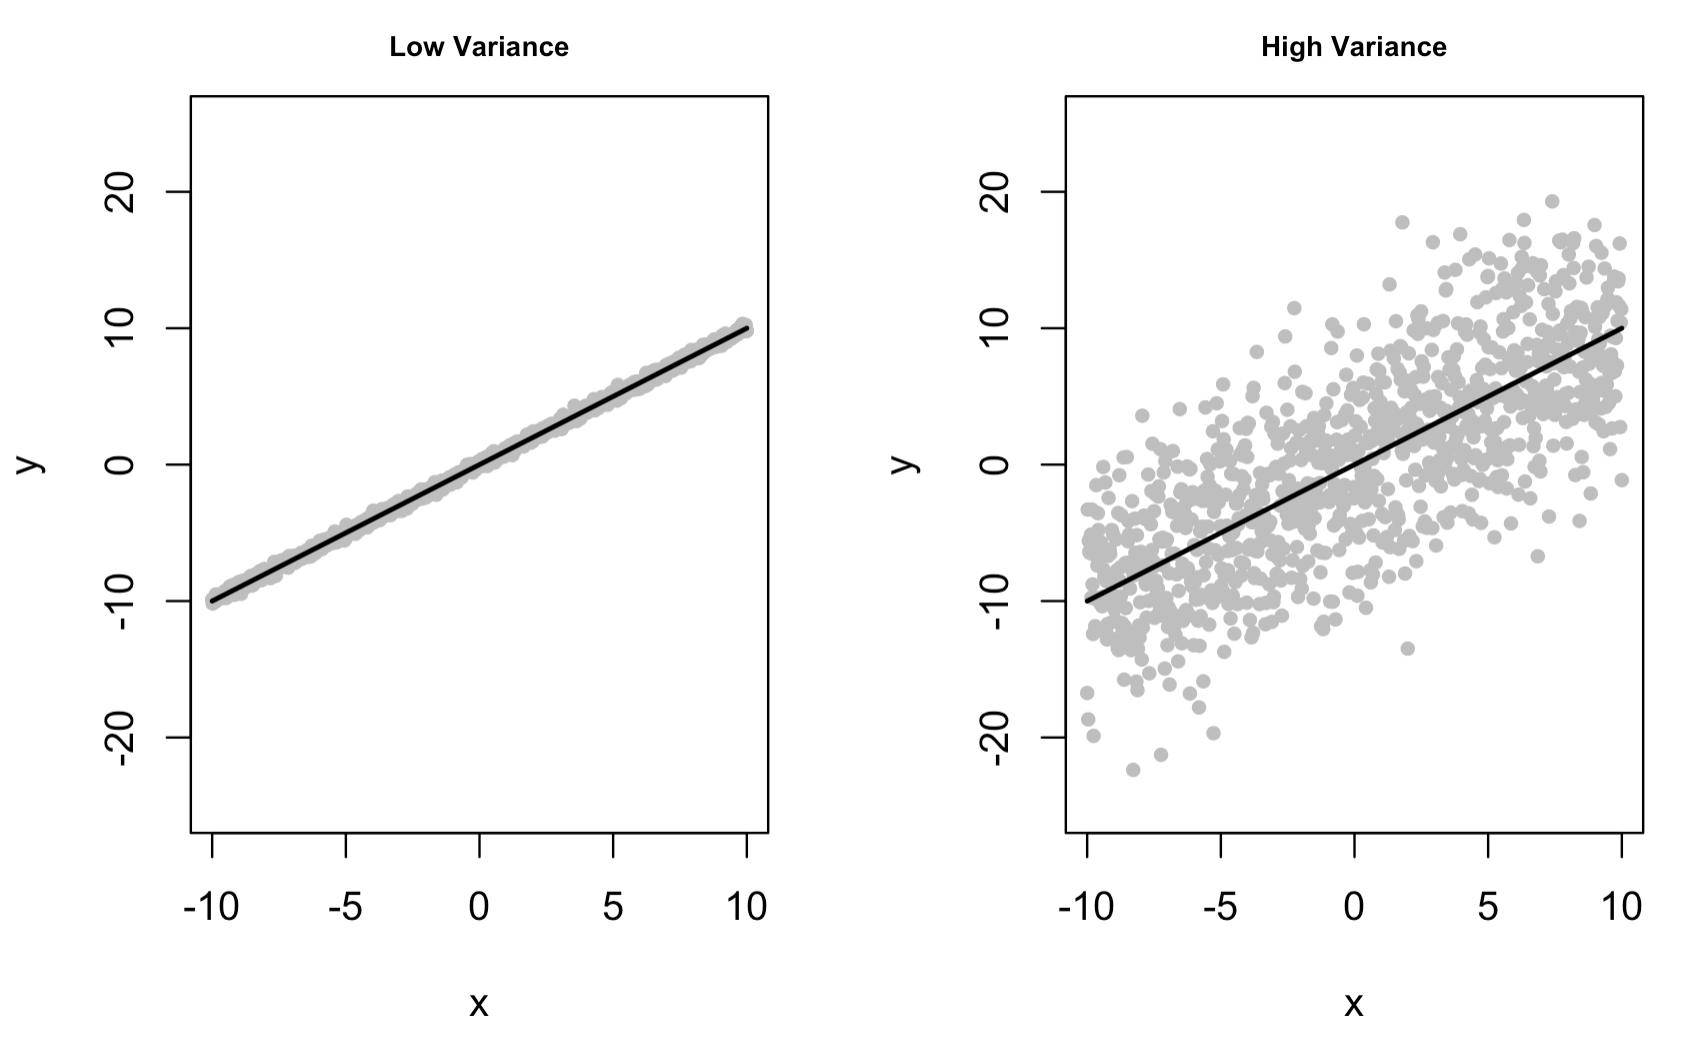
\includegraphics[width = 0.7\textwidth]{variance}
\end{center}
\end{frame}

\begin{frame}{SGD -- Why Variance Matters}
\textbf{Self-tuning}
\begin{center}
	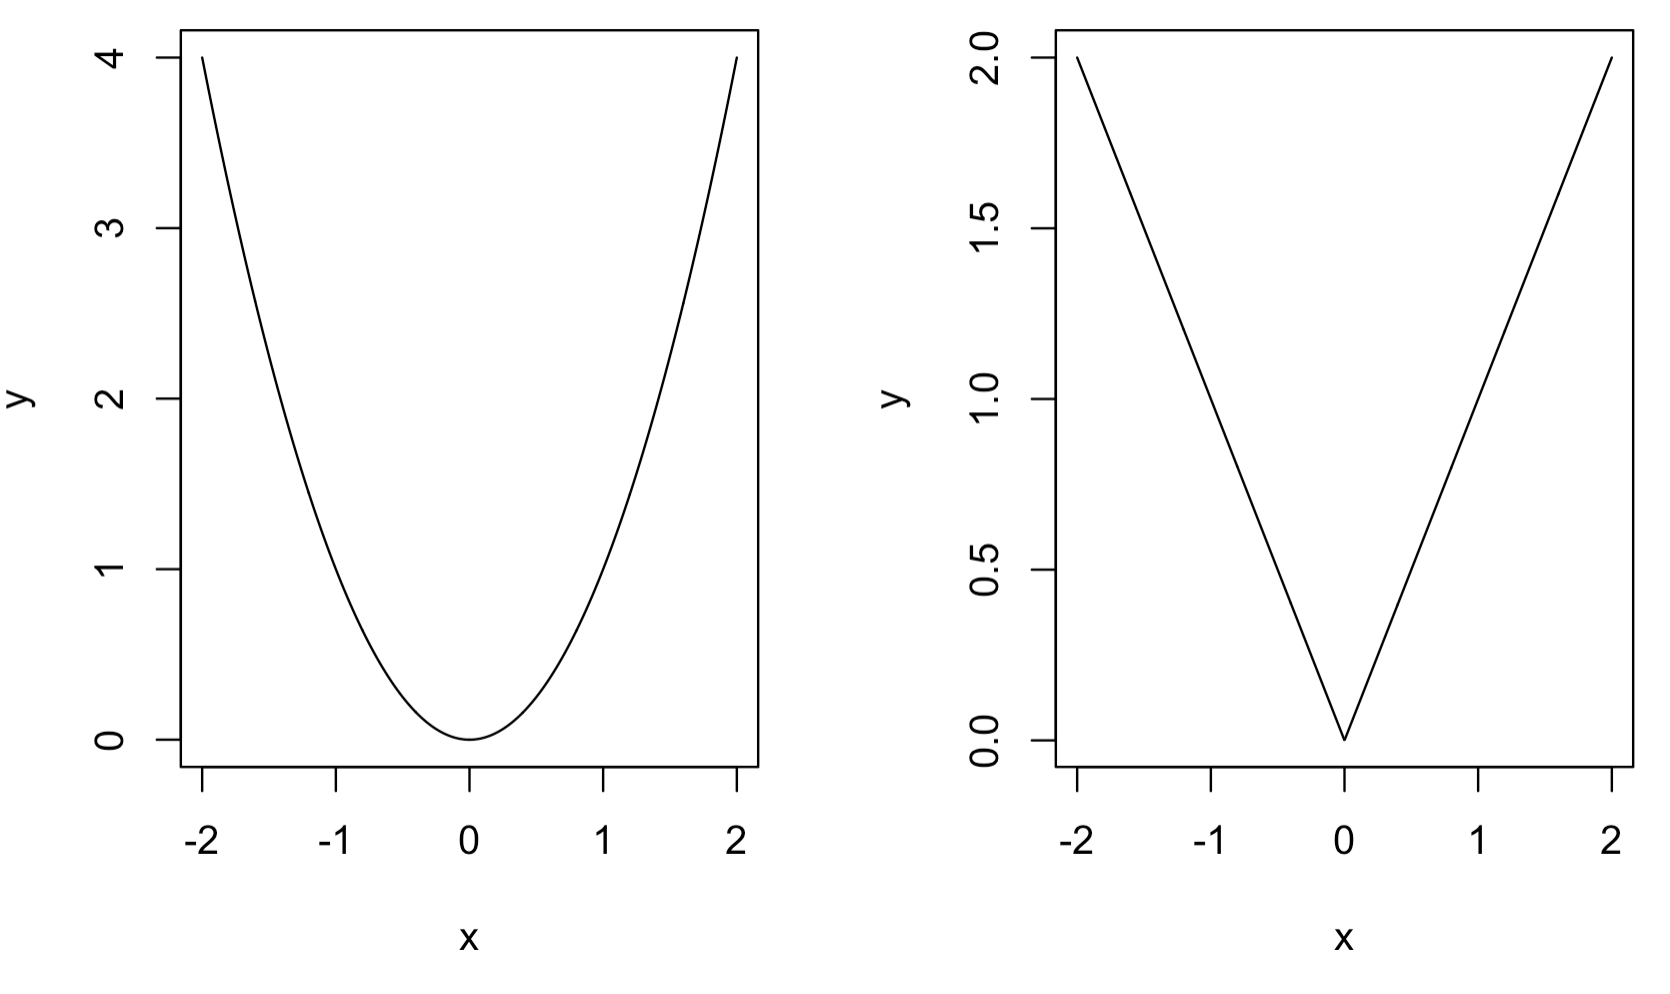
\includegraphics[width = 0.6\textwidth]{selftuning}
\end{center}
\begin{center}
	When Polyak-Lojasiewicz Inequality hold, $x \to x^*$, $\nabla f(x) \to 0$
\end{center}
\end{frame}

%------------------------------------------------

\begin{frame}{SGD}

\begin{block}{Theorem: Convergence Rate}

Suppose $x^*$ exists, and $E_\xi[||\tilde g(x)||^2] \le G^2\ \ \forall x$.
\begin{equation*}
	x_{t+1} = x_t - \eta \tilde g(x)
\end{equation*}

then 

\begin{equation*}
	E_\xi[f(\frac{1}{T} \sum_{t = 1}^T x_t)] - f(x^*) \le \frac{R G^2}{\sqrt T}
\end{equation*}

$$R^2 \ge ||x_1 - x^* ||_2$$

\end{block}


\end{frame}

%------------------------------------------------

\begin{frame}{SGD}


\begin{block}{Theorem: Convergence Rate}

Suppose $x^*$ exists, and $E[||\tilde g(x)||^2] \le G^2\ \ \forall x$, and $f$ is $\mu$ strongly convex, may not be smooth, then SGD with decreasing step size $\eta_t = \frac{2}{\mu (t + 1)}$
\begin{equation*}
	x_{t+1} = x_t - \eta_t \tilde g(x)
\end{equation*}

then 

\begin{equation*}
	E[f(\frac{2t}{T(T+1)} \sum_{t = 1}^T x_t)] - f(x^*) \le \frac{2 G^2}{\mu} \frac{1}{T+1} = \mathcal O(\frac{1}{T})
\end{equation*}


\end{block}


	
\end{frame}

%------------------------------------------------

\begin{frame}{Quick Summary}
	\begin{itemize}[<+->]
		\item convergence rate = $\mathcal O(\frac{1}{\sqrt T})$ when $E[||\tilde g||_2^2] \le G^2$
		\item convergence rate = $\mathcal O(\frac{1}{ T})$ when we have strong convexity
	\end{itemize}
	\
	
	\
	
	\textbf{Question:} Can we go a little bit better, what's the key?
	
\pause \begin{center}
	self-tuning property
\end{center}
\end{frame}

%------------------------------------------------

\begin{frame}{Two Ways To Reduce Variance}
\Large
\begin{itemize}
	\item Mini-Batch 
	\item Recentering
\end{itemize}
	
\end{frame}

%------------------------------------------------

\begin{frame}{Convergence Rate of SGD}

\begin{align*}
	&x_{t+1} = x_t - \eta \nabla f_I(x_t) \\
	&E(\frac{1}{T}\sum_{i=1}^T x_t ) - f(x^*) \le \frac{RG^2}{\sqrt{T}} \le \frac{||x_1 - x^*||}{\sqrt T} \sqrt{E[||\nabla f_I(x)||_2^2]}
\end{align*}
\quad \quad \quad \quad \quad \quad \quad  Recall that $R \le ||x_1 - x^*||$, and $E[||\nabla f_I(x)||_2^2] \le G^2$

\

\begin{center}
	\pause \textbf{Question:} Can we control $\sqrt{E[||\nabla f_I(x)||_2^2]}$?
\end{center}

	
\end{frame}

%------------------------------------------------

\begin{frame}{Mini-Batch SGD}
\begin{align*}
	x \Longrightarrow \Box \Longrightarrow \xout{\nabla f(x)} \Longrightarrow \tilde g(x) = \frac{1}{B}\sum_{j = 1}^B \nabla f_{I_j}(x)
\end{align*}
$$I_j \sim \text{uniform}(1, 2, \ldots, n)$$

\textbf{Question:} is $\tilde g(x)$ stochastic gradient?

\pause check: $$E_I[\frac{1}{B} \sum_{j=1}^B\nabla f_{I_j}(x)] = \frac{1}{B}\sum_{j = 1}^B \nabla f(x) = \nabla f(x)$$

\textbf{Does it help?}

assume variance is independent,

$$Var(\frac{1}{B}\sum_{j=1}^B \nabla f_{Ij}(x)) = \frac{1}{B^2}\sum_{j=1}^B Var(f_{I_j}(x)) = \frac{1}{B}Var(f_{I_j}(x))$$

\end{frame}

%------------------------------------------------

\begin{frame}{Mini-Batch SGD}
\textbf{Advantages}
\begin{itemize}
	\item reduce variance
	\item mini-batch is parallelizable
\end{itemize}


\textbf{Disadvantages}

\begin{itemize}
	\item more work per iteration
	\item no self-tunning when the $f$ is smooth
\end{itemize}

\pause \textbf{Question:} can we do better?

\

\pause We need self-tuning when $f$ smooth and strongly convex

\end{frame}


%------------------------------------------------

\begin{frame}{Reduce Variance by Recentering}
	For $x$ and $y$
	
\begin{align*}
	x, y \Longrightarrow \Box \Longrightarrow \xout{\nabla f(x)} \Longrightarrow \tilde g(x) = \nabla f_I(x) - (\nabla f_I(y) - \nabla f(y))
\end{align*}

$$I \sim \text{uniform}(1, 2, \ldots, n)$$

\begin{align*}
	E_I[\tilde g(x)] & = E_I[\nabla f_I(x) - (\nabla f_I(y) - \nabla f(y))]\\
	& = \nabla f(x) \cancelto{0}{\bcancel{- (\nabla f(y) - \nabla f(y))}}
\end{align*}

	
\end{frame}



%------------------------------------------------

\begin{frame}{Stochastic Variance Reduced Gradient Descent Algorithm (SVRG)}
\textbf{Outer Loop:}\\
\hspace{1cm} On the $k^{th}$ iteration \\
\hspace{1cm} $x_1 = y_k$\\
\hspace{1cm} \textbf{Inner Loop:}\\
\hspace{2cm} for $t = 1,2,\ldots T$\\
\hspace{3cm} $x_{t+1} = x_t - \eta\Big( \nabla f_I(x_t) - \big(\nabla f_I(y_k) - \nabla f(y_k)\big) \Big)$\\
\
\hspace{2cm} update $y_{k+1} = \frac{1}{T}\sum_{i=1}^T x_t$, and compute $\nabla f(y_{k+1})$

\begin{itemize}
	\item inner loop only compute $\nabla f_I(x_t)$
	\item outter loop compute full gradient $\nabla f(y_{k+1})$
\end{itemize}

\end{frame}



%------------------------------------------------

\begin{frame}{Variance Reduction Lemma}

\begin{block}{Variance Reduction Lemma}
	Let $f_1 \ldots f_n$ be L-smooth, $I \sim \text{uniform}(1,\ldots n)$.
	Then $E_I\Big[|| \nabla f_I(x) - \nabla f_I(x^*)  ||_2^2\Big] \le 2L (f(x) - f(x^*))$
\end{block}

\textbf{Note:} $\nabla f_I(x)$ may not be small when $x \to x^*$

\end{frame}


%------------------------------------------------

\begin{frame}{Proof of Variance Reduction Lemma}

Let $g_i(x) = f_i(x) - [ f_i(x^*) + \nabla f_i(x^*)^T(x - x^*) ] \ge 0$ by convextiy

\

If $h$ is convex and $L$-smooth, $h(x - \frac{1}{L} \nabla h(x) ) \le h(x) - \frac{1}{2L}||\nabla h(x)||_2^2$ and applies this to $g$

\begin{align*}
	&0 \le g_i(x - \frac{1}{L} \nabla g_i(x) ) \le g_i(x) - \frac{1}{2L}||\nabla g_i(x)||_2^2 \\
	&\hspace{2cm} \downarrow\\
	&-g_i(x) \le - \frac{1}{2L}||\nabla g_i(x)||_2^2 \\
	&\hspace{2cm} \downarrow\\
	&||\nabla g_i(x)||_2^2  \le 2L g_i(x)
\end{align*}
	
\end{frame}




%------------------------------------------------

\begin{frame}{Proof of Variance Reduction Lemma -- Continuous}


\begin{align*}
	&g_i(x) = f_i(x) - [ f_i(x^*) + \nabla f_i(x^*)^T(x - x^*) ] \ge 0 \\
	&||\nabla g_i(x)||_2^2 = || \nabla f_i(x) - \nabla f_i(x^*)||_2^2 \le 2L \Big(f_i(x) - f_i(x^*) + \nabla f_i(x^*)^T(x - x^*) \Big)\\
	& E_I\Big[||\nabla f_I(x) - \nabla f_I(x^*)||\Big] \le 2L E\Big[ f_I(x) - f_I(x^*) + \nabla f_I(x^*)^T(x - x^*) \Big]\\
	& \hspace{38.5mm} \le 2L\Big( f(x) - f(x^*) + \cancelto{0}{\nabla f(x^*)^T} (x - x^*) \Big) 
\end{align*}

The recentered gradient $E_I\Big[||\nabla f_I(x) - \nabla f_I(x^*)||\Big] \to 0$, when $x \to x^*$

\end{frame}

%------------------------------------------------

\begin{frame}{Stochastic Variance Reduction Griadent Desecent}
	\begin{block}{SVRG Theorem}
	Let $f = \frac{1}{n}\sum_{i=1}^n f_i(x)$, $f_i$ is $L$-smooth, and $f$ is $\mu$ strongly convex. SVRG algorithm with step size $\eta = \frac{1}{10 \cdot L}$, and inner loop size $T = 10 \cdot (\frac{L}{\mu})$.
	
	Then after $s+1$ iterations of the outer loop
	\begin{equation*}
		E[f(y^{s+1})] - f(x^*) \le 0.9^s(f(y^1) - f(x^*))
	\end{equation*}
	\end{block}
\textbf{Key Feature:}

\begin{itemize}
	\item linear convergence
	\item $L/\mu$ does not appear in the convergence rate
\end{itemize}	
\end{frame}

%------------------------------------------------


\begin{frame}{Proof of SVRG Algorithm}
	good enough to prove $E[f(y^{s+1})] - f(x^*) \le 0.9(f(y^s) - f(x^*))$
	
	\
	
	\textbf{Recall:} $y^{s+1} = \frac{1}{T} \sum x_t$, where $x_t$ is provided in $s^{th}$ inner loop
	\begin{align*}
		\Big|\Big|x_{t+1} - x^*\Big|\Big|_2^2 &= \Big|\Big| x_t - \eta \Big(\nabla f_{I_t}(x_t) - \big(\nabla f_{I_t}(y) - \nabla f(y)\big) \Big) - x^*\Big|\Big|_2^2\\
		& = || x_t - x^*||_2^2 - 2\eta \underbrace{\Big(\nabla f_{I_t}(x_t) -\nabla f_{I_t}(y) + \nabla f(y) \Big)^T}_{V_t}(x_t - x^*) + \eta^2 ||V_t|||_2^2 \\
		& = \underbrace{|| x_t - x^*||_2^2}_{a} - \underbrace{2\eta V_t^T(x_t - x^*)}_{b} + \underbrace{ \overbrace{\eta^2 ||V_t||_2^2}^{\text{variance term}} }_{c}
	\end{align*}
	$a\to 0$ and $b \to 0$ when $x_t \to x^*$, we want the term $c$ goes to 0 as well 
\end{frame}

%------------------------------------------------


\begin{frame}{Proof of SVRG Algorithm}
Let's just look at the term $c$

\begin{align*}
	E\Big[\big|\big|V_t\big|\big|_2^2\Big] &= E\Big[ \big|\big|\nabla f_{I_t}(x_t) - \nabla f_{I_t}(y) + \nabla f(y)\big|\big|_2^2\Big] \\
	&= E\Big[ \big|\big|\nabla f_{I_t}(x_t) - \nabla f_{I_t}(x^*) + \nabla f_{i_t}(x^*) - \nabla f_{i_t}(y) + \nabla f(y)\big|\big|_2^2\Big]\\
	& \le 2E\Big[\big|\big| \nabla f_{I_t}(x_t) - \nabla f_{I_t}(x^*)  \big|\big|_2^2\Big] + \underbrace{2E\Big[\big|\big| \nabla f_{I_t}(x^*) - \nabla f_{I_t}(y) + \nabla f(y) \big|\big|_2^2\Big]}_{=0}\\
	& \le 2E\Big[\big|\big| \nabla f_{I_t}(x_t) - \nabla f_{I_t}(x^*)  \big|\big|_2^2\Big] + 2E\Big[\big|\big|   \nabla f_{I_t}(y) - f_{I_t}(x^*)   \big|\big|_2^2\Big]\\
	& \le 4L(f(x_t) - f(x^*) + f(y) - f(x^*) ) \quad \text{by variance reduction lemma twice}
\end{align*}

\pause ps $E[(Y - E(Y))^2] \le E[Y^2]$

\end{frame}

%------------------------------------------------


\begin{frame}{Proof of SVRG Algorithm}

term b
\begin{align*}
	E\Big[2\eta V_t^T(x_t - x^*)\Big] &= 2\eta E[V_t]^T(x_t - x^*)\\
	& = 2\eta \nabla f(x_t)^T(x_t - x^*)\\
	& \ge 2\eta \big( f(x_t) - f(x^*) \big) \quad \text{by convexity}
\end{align*}
Then, we have
\begin{align*}
	E\Big[ || x_{t+1} - x^* ||_2^2 \Big] &= E[a + b + c]\\
	& \le ||x_t - x^* ||_2^2 - 2\eta \big( f(x_t) - f(x^*) \big) + 4\eta^2 L(f(x_t) - f(x^*) + f(y) - f(x^*) ) \\
	& = ||x_t - x^* ||_2^2 - 2\eta(1 - 2\eta L)(f(x_t) - f(x^*)) + 4\eta^2L(f(y) - f(x^*))\\
	& \hspace{58mm} \downarrow \text{iterating}\\
	& = ||x_1 - x^*||_2^2 - 2\eta(1-2\eta L)\cdot E[\sum_{k=1}^t (f(x_k) - f(x^*)) ] + 4\eta^2L\cdot t(f(y) - f(x^*))
\end{align*}

\end{frame}


%------------------------------------------------

\begin{frame}{Proof of SVRG Algorithm}
\textbf{Recall:}
\begin{itemize}
	\item $x_1 = y^k$
	\item $||y - x^*||_2^2 \le \frac{2}{\mu}(f(y) - f(x^*))$
\end{itemize}

\begin{align*}
	&E\Big[ || x_{t+1} - x^* ||_2^2 \Big]  \le ||x_1 - x^*||_2^2 - 2\eta(1-2\eta)L\cdot E[\sum_{k=1}^t (f(x_k) - f(x^*)) ] + 4\eta^2L\cdot t(f(y) - f(x^*))\\
	&2\eta(1-2\eta)L\cdot E[f(\frac{1}{T}\sum x_t) - f(x^*) ] \le (\frac{2}{\mu} + \eta^24LT ) \frac{1}{T} E(f(y) - f(x^*)) \\
	& E[f(y^{s+1})] - f(x^*) \le 0.9 \big( E[f(y^s)] - f(x^*)\big)
\end{align*}


\end{frame}

%------------------------------------------------

%------------------------------------------------
\section{Momentum Acceleration}
%------------------------------------------------


\begin{frame}{Accelerate Gradient Descent}
\large
\textbf{Key Idea}: 
use gradient computed at previous step to accelerate the algorithm

\

\textbf{Methods}:

	\begin{itemize}
		\item Momentum
		\item Nesterov
	\end{itemize}

\end{frame}


%------------------------------------------------

\begin{frame}{Momentum Acceleration}
\textbf{Momentum Method:}
	\begin{align*}
		&x_{k+1} = x_k - \eta z_k\\
		&z_k = \nabla f(x_k) + \beta z_{k-1}
	\end{align*}
\textbf{Nesterov Method:}
\begin{align*}
	&x_{t+1} = x_t + d_t - \eta \nabla f(x_t + d_t)\\
	&d_t = \gamma_t (x_t - x_{t-1})
\end{align*}

\begin{block}{Theorem}
Let $f$ to be $L$-smooth and $\mu$-convex.
\begin{equation*}
	f(z_t) - f(x^*) \le \frac{L + \mu}{2} ||x_1 -x^* ||_2^2\cdot \exp\{ \frac{(t+1)}{\sqrt{k}} \}
\end{equation*}
	
\end{block}

\end{frame}



%------------------------------------------------


\begin{frame}{Summary}

\begin{itemize}
	\item gradient descent: $\mathcal O(n\frac{L}{\mu} \log(\frac{1}{\epsilon}))$ iterations for $\epsilon$-accuracy 
	\item momentum acceleration: $\mathcal O(n\sqrt{\frac{L}{\mu} }\log(\frac{1}{\epsilon}))$ iterations for $\epsilon$-accuracy 
	\item stochastic gradient descent: $\mathcal O(\frac{1}{\mu\epsilon})$ for $\epsilon$-accuracy
	\item SVRG: $\mathcal O((n + \frac{L}{\mu})\log(\frac{1}{\varepsilon}))$ for $\epsilon$-accuracy
\end{itemize}


	
\end{frame}


%------------------------------------------------
%------------------------------------------------
%------------------------------------------------

%------------------------------------------------

\begin{frame}
    \Huge{\centerline{\textbf{The End}}}
\end{frame}

%----------------------------------------------------------------------------------------

\end{document}mu